\documentclass[
11pt, % The default document font size, options: 10pt, 11pt, 12pt
codirector, % Uncomment to add a codirector to the title page
]{charter} 




% El títulos de la memoria, se usa en la carátula y se puede usar el cualquier lugar del documento con el comando \ttitle
\titulo{Sistema de riego y control de huertas} 

% Nombre del posgrado, se usa en la carátula y se puede usar el cualquier lugar del documento con el comando \degreename
%\posgrado{Carrera de Especialización en Sistemas Embebidos} 
\posgrado{Carrera de Especialización en Internet de las Cosas} 
%\posgrado{Carrera de Especialización en Intelegencia Artificial}
%\posgrado{Maestría en Sistemas Embebidos} 
%\posgrado{Maestría en Internet de las cosas}

% Tu nombre, se puede usar el cualquier lugar del documento con el comando \authorname
\autor{Lic. Siciliano Gustavo Hernan} 

% El nombre del director y co-director, se puede usar el cualquier lugar del documento con el comando \supname y \cosupname y \pertesupname y \pertecosupname
\director{Mg. Ing. Osvaldo Ivani}
\pertenenciaDirector{FIUBA} 
% FIXME:NO IMPLEMENTADO EL CODIRECTOR ni su pertenencia
\codirector{Codirector a definir} % para que aparezca en la portada se debe descomentar la opción codirector en el documentclass
\pertenenciaCoDirector{FIUBA}

% Nombre del cliente, quien va a aprobar los resultados del proyecto, se puede usar con el comando \clientename y \empclientename
\cliente{Alejandra Vranic}
\empresaCliente{Universidad Nacional de Lanús}

% Nombre y pertenencia de los jurados, se pueden usar el cualquier lugar del documento con el comando \jurunoname, \jurdosname y \jurtresname y \perteunoname, \pertedosname y \pertetresname.
\juradoUno{Jurado a definir}
\pertenenciaJurUno{FIUBA} 
\juradoDos{Jurado a definir}
\pertenenciaJurDos{FIUBA}
\juradoTres{Jurado a definir}
\pertenenciaJurTres{FIUBA}
 
\fechaINICIO{20 de octubre de 2022}		%Fecha de inicio de la cursada de GdP \fechaInicioName
\fechaFINALPlan{8 de diciembre de 2022} 	%Fecha de final de cursada de GdP
\fechaFINALTrabajo{a definir}	%Fecha de defensa pública del trabajo final


\begin{document}

\maketitle
\thispagestyle{empty}
\pagebreak


\thispagestyle{empty}
{\setlength{\parskip}{0pt}
\tableofcontents{}
}
\pagebreak


\section*{Registros de cambios}
\label{sec:registro}


\begin{table}[ht]
\label{tab:registro}
\centering
\begin{tabularx}{\linewidth}{@{}|c|X|c|@{}}
\hline
\rowcolor[HTML]{C0C0C0} 
Revisión & \multicolumn{1}{c|}{\cellcolor[HTML]{C0C0C0}Detalles de los cambios realizados} & Fecha      \\ \hline
0      & Creación del documento                                 &\fechaInicioName \\ \hline
1      & Se completa hasta la sección 5 inclusive                 & 2 de noviembre de 2022 \\ \hline
2      & Se aplican las correcciones de la primera entrega                 & 6 de noviembre de 2022 \\ \hline
3      & Se completa hasta la sección 9 inclusive                 & 9 de noviembre de 2022 \\ \hline
4      & Se aplican las correcciones de la segunda entrega                 & 14 de noviembre de 2022 \\ \hline
5      & Se agrega la información del director del trabajo                & 15 de noviembre de 2022 \\ \hline
6      & Se completa hasta la sección 12 inclusive                 & 16 de noviembre de 2022 \\ \hline
7      & Se aplican las correcciones de la tercera entrega
& 22 de noviembre de 2022 \\ \hline
8      & Se finaliza el documento completando hasta la sección 15 inclusive & 24 de noviembre de 2022 \\ \hline
9      & Se aplican las correcciones de la última entrega & 27 de noviembre de 2022 \\ \hline

\end{tabularx}
\end{table}

\pagebreak



\section*{Acta de constitución del proyecto}
\label{sec:acta}

\begin{flushright}
Buenos Aires, \fechaInicioName
\end{flushright}

\vspace{2cm}

Por medio de la presente se acuerda con el \authorname\hspace{1px} que su Trabajo Final de la \degreename\hspace{1px} se titulará ``\ttitle'', el cual consistirá esencialmente en la implementación de un prototipo de monitoreo de humedad y riego automático de huertas. Tendrá un presupuesto preliminar estimado de {600} horas de trabajo y {\$80.388,1 pesos argentinos} para la compra de materiales, con fecha de inicio \fechaInicioName\hspace{1px} y fecha de presentación pública \fechaFinalName.

Se adjunta a esta acta la planificación inicial.

\vfill

% Esta parte se construye sola con la información que hayan cargado en el preámbulo del documento y no debe modificarla
\begin{table}[ht]
\centering
\begin{tabular}{ccc}
\begin{tabular}[c]{@{}c@{}}Dr. Ing. Ariel Lutenberg \\ Director posgrado FIUBA\end{tabular} & \hspace{2cm} & \begin{tabular}[c]{@{}c@{}}Mg. \clientename \\ \empclientename \end{tabular} \vspace{2.5cm} \\ 
\multicolumn{3}{c}{\begin{tabular}[c]{@{}c@{}} \supname \\ Director del Trabajo Final\end{tabular}} \vspace{2.5cm} \\
%\begin{tabular}[c]{@{}c@{}}\jurunoname \\ Jurado del Trabajo Final\end{tabular}     &  & \begin{tabular}[c]{@{}c@{}}\jurdosname\\ Jurado del Trabajo Final\end{tabular}  \vspace{2.5cm}  \\
%\multicolumn{3}{c}{\begin{tabular}[c]{@{}c@{}} \jurtresname\\ Jurado del Trabajo Final\end{tabular}} \vspace{.5cm}                                                                     
\end{tabular}
\end{table}




\section{1. Descripción técnica-conceptual del proyecto a realizar}
\label{sec:descripcion}


\begin{consigna}{black} % El bloque "consigna" se usa para poner texto en rojo y dar una pequeña ayuda sobre cómo completar la sección

El presente trabajo nace a partir de un proyecto de investigación originado en la UNLa (Universidad Nacional de Lanús) y consiste en el desarrollo de un prototipo tecnológico que pueda medir el porcentaje de humedad de un conjunto de plantas en una huerta. Además, se implementará un software de seguimiento y control de las mediciones.

La finalidad del proyecto es contar con un sistema de monitoreo de huertas que colabore con mantener condiciones optimas para los cultivos. Esto se logrará tanto con revisiones manuales de las métricas obtenidas, como con el sistema de riego automático. Este último activará una válvula de agua que conseguir un buen cuidado de las plantas.
En base a esto se proyecta que una huerta va a estar compuesta por varios sectores. En cada uno se van a agrupar plantas con características de cuidado similares. Además, cada sector contará con un prototipo con una placa ESP32 y dos sensores para medir el porcentaje de humedad del suelo y del ambiente. Las placas deberán tener conexión Wi-Fi para enviar las métricas al Backend del servidor vía protocolo HTTP. Ese sistema va a nutrir una plataforma Web. En el Frontend habrá un panel de administración por sector, para que en cada uno se puedan fijar valores mínimos de porcentaje de humedad. En caso de que las mediciones sean inferiores a estos valores de control, el Backend generará un mensaje para los dispositivos. De esta manera se accionará la manguera de riego y se podrá tener un cuidado simple y automático de las plantas.


%\vspace{25px}

\begin{figure}[htpb]
\centering 
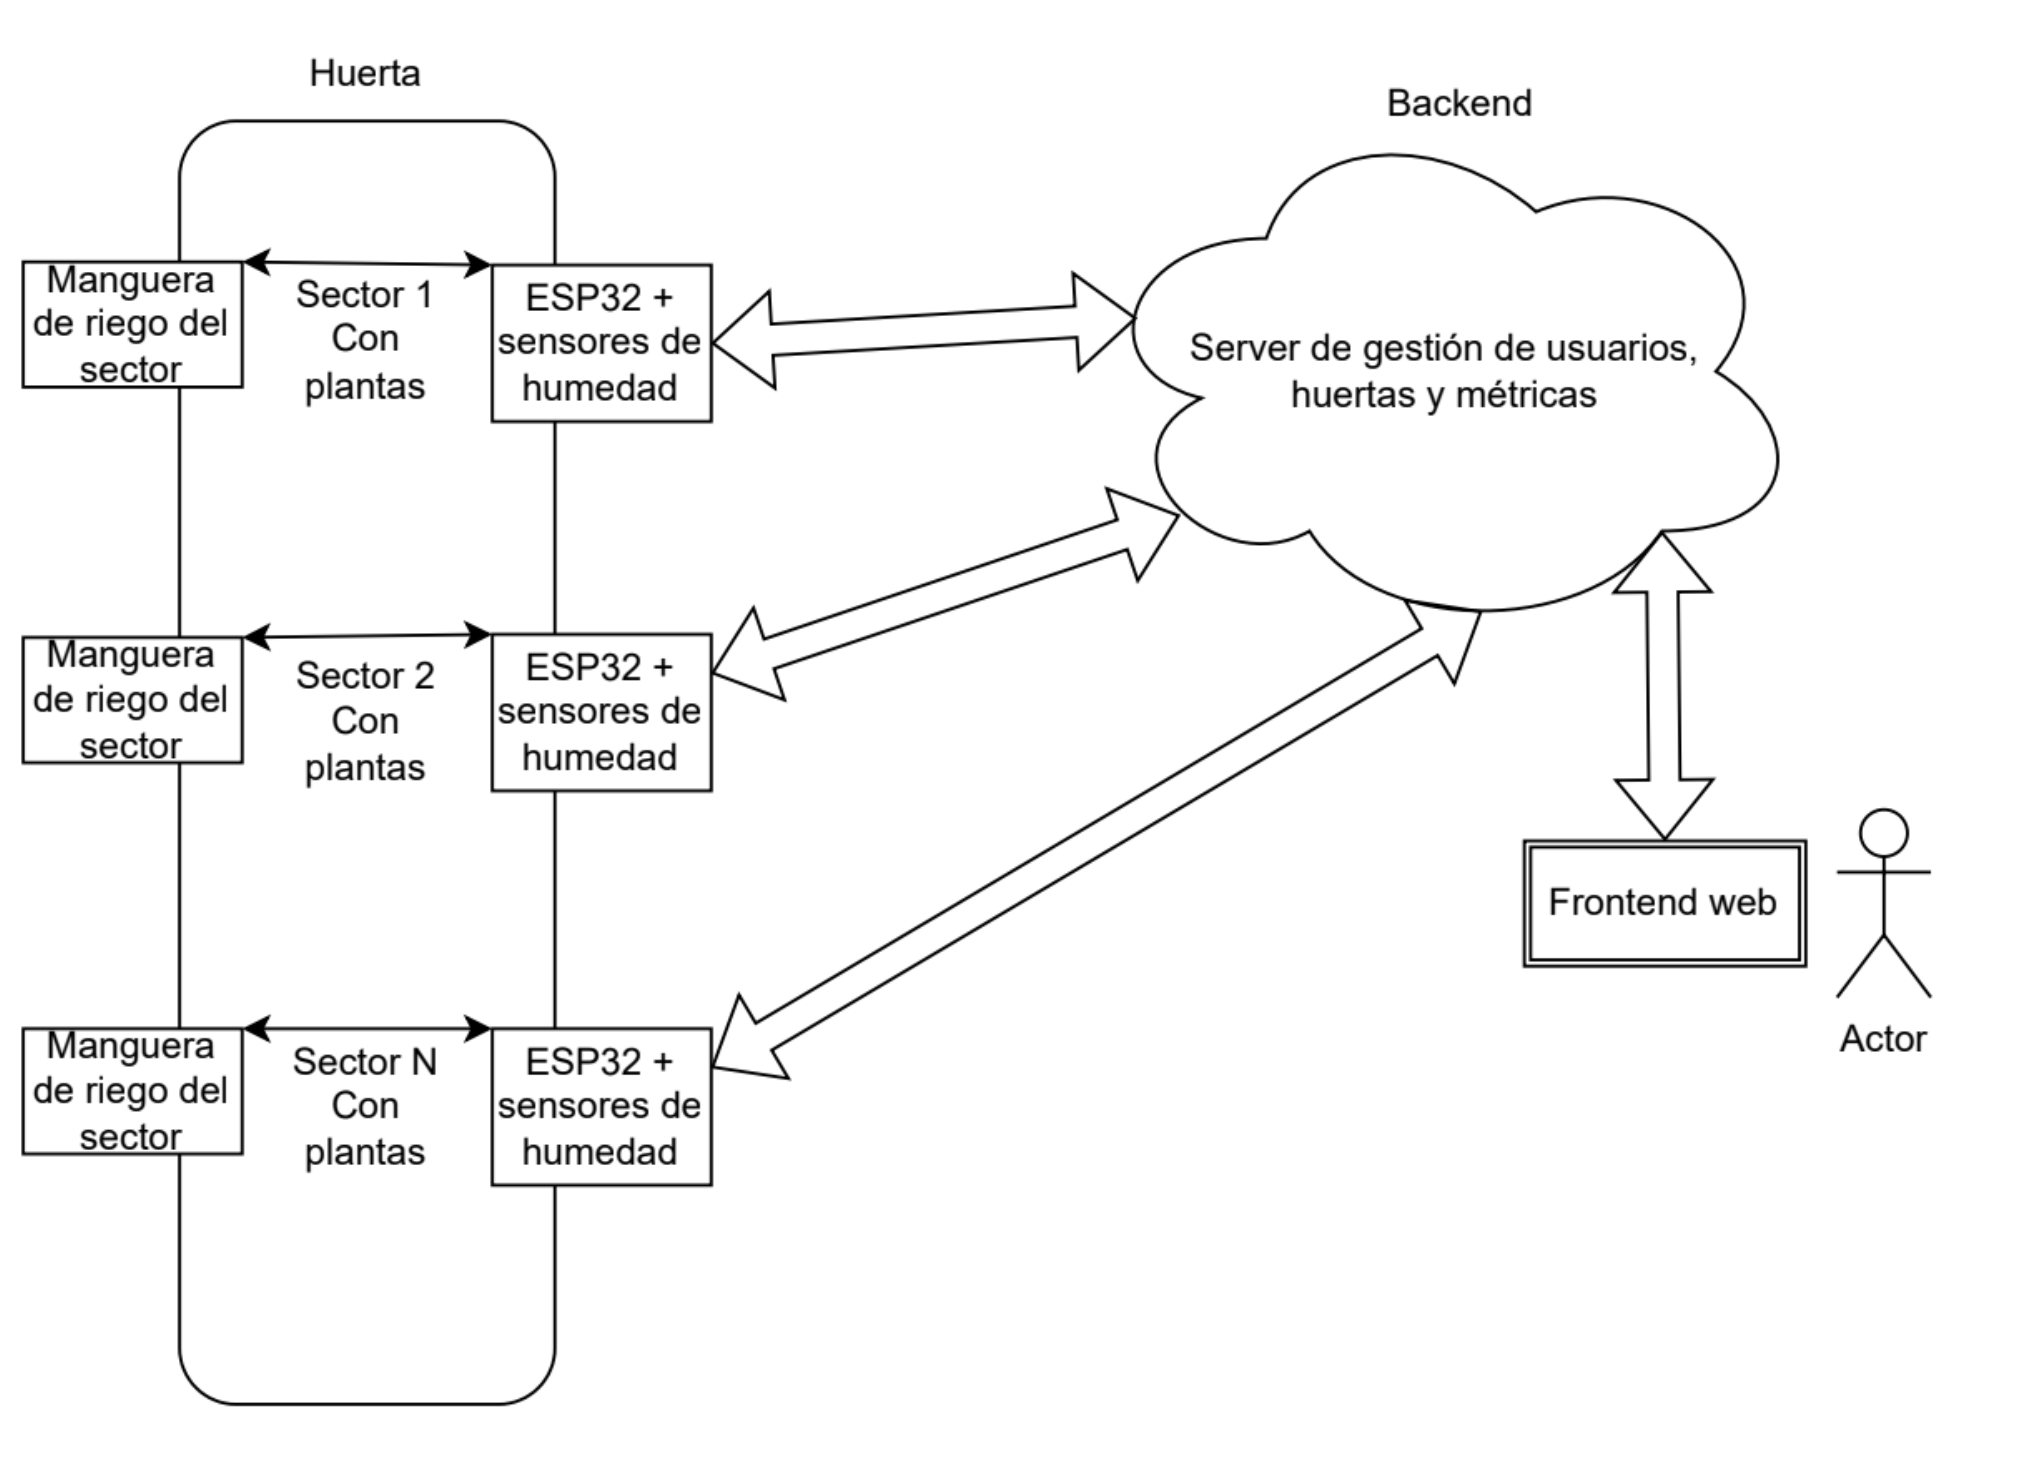
\includegraphics[width=.9\textwidth]{./Figuras/diagBloques.png}
\caption{Diagrama del sistema.}
\label{fig:diagBloques}
\end{figure}

\vspace{25px}

\end{consigna}


\section{2. Identificación y análisis de los interesados}
\label{sec:interesados}

\begin{consigna}{black} 

\begin{table}[ht]
%\caption{Identificación de los interesados}
%\label{tab:interesados}
\begin{tabularx}{\linewidth}{@{}|l|X|X|l|@{}}
\hline
\rowcolor[HTML]{C0C0C0} 
Rol&
Nombre y Apellido&
Organización&
Puesto\\ \hline

Auspiciante&
\clientename &
\empclientename &
Directora de la Licenciatura en Sistemas\\ \hline

Cliente&
\clientename &
\empclientename & 
Directora de la Licenciatura en Sistemas\\ \hline

Impulsor&
Laura Loidi&
\empclientename &
Coordinadora de proyectos de investigación\\ \hline

Responsable&
\authorname &
FIUBA&
Alumno\\ \hline

Colaboradores&
Leandro Rios&
\empclientename &
Docente investigador\\ \hline

Orientador&
\supname &
\pertesupname &
Director de trabajo final\\ \hline

Equipo&
-Reboredo Damian\newline 
-Contento Guido\newline
-Otegui Luciano&
\empclientename &
Estudiantes investigadores\\ \hline

Usuario final&
Estudiantes UNLa y Vallese&
\empclientename &
Estudiantes\\ \hline
\end{tabularx}
\end{table}


\begin{itemize} 
	\item Cliente: Alenadra Vranic (que también oficia como Auspiciante) necesita tener un plan de trabajo para Diciembre 2022 y avances trimestrales duramente 2023.
	\item Impulsor: Laura Loidi en su rol de coordinadora de proyectos de investigación dará asistencia y seguimiento metodológico.	
	\item Colaborador: Leandro Rios va a dar soporte para la compra, armado e instalación de los dispositivos en la huerta.
	\item Equipo: los estudiantes finalizarán sus tareas de investigación entre diciembre del 2022 y febrero del 2023. Se tiene que delimitar el alcance y las futuras líneas de desarrollo para este trabajo para fines de noviembre del 2022.
	\item Orientador: aún se definió el director del trabajo. Esto tiene que resolverse antes de la quinta clase de Gestión de Proyectos.
\end{itemize}

\end{consigna}



\section{3. Propósito del proyecto}
\label{sec:proposito}

\begin{consigna}{black}

El propósito de este proyecto es generar un rédito intelectual, económico y cultural dentro de la UNLa. Para cumplir esto se tienen 4 verticales principales de trabajo:

1- Armar un prototipo técnico para tomar mediciones de las plantas en una huerta. Con esos valores se deberá operar una manguera de agua y brindar métricas del estado de los cultivos.

2- Desarrollar un software web que pueda tomar las métricas del prototipo y gestionarlas a través de un panel de control.

3- Implementar en la escuela oficios de Felipe Vallese (http://oficios.unla.edu.ar), y en la UNLa, una serie de huertas que sirvan para dar empleo y nutrir de alimentos estas organizaciones y a escuelas aledañas.

4- Consolidar un curso que conste de capacitaciones a darse en Felipe Vallese. La idea es extender el conocimiento de cómo montar el prototipo para personas de la comunidad.
Como un punto extra, el material generado en el proyecto también se podría utilizar para incluir una materia optativa en la carrera de Licenciatura en Sistemas de la UNLa.


\end{consigna}

\section{4. Alcance del proyecto}
\label{sec:alcance}

\begin{consigna}{black}

El presente proyecto tiene como alcance trabajar en las verticales 1, 2 y 3 de la sección anterior.

En relación al punto 1, se completará el prototipo inicial de la placa ESP32 con sus dos sensores. Este trabajo se está llevando adelante con el estudiante Damian Reboredo. Actualmente ya se cuenta con una versión funcional que no contempla a la manguera con una conexión de agua. Se deberá finalizar esa tarea, más la integración con el sistema de control y monitoreo.

%\vspace{25px}

\begin{figure}[htpb]
\centering 
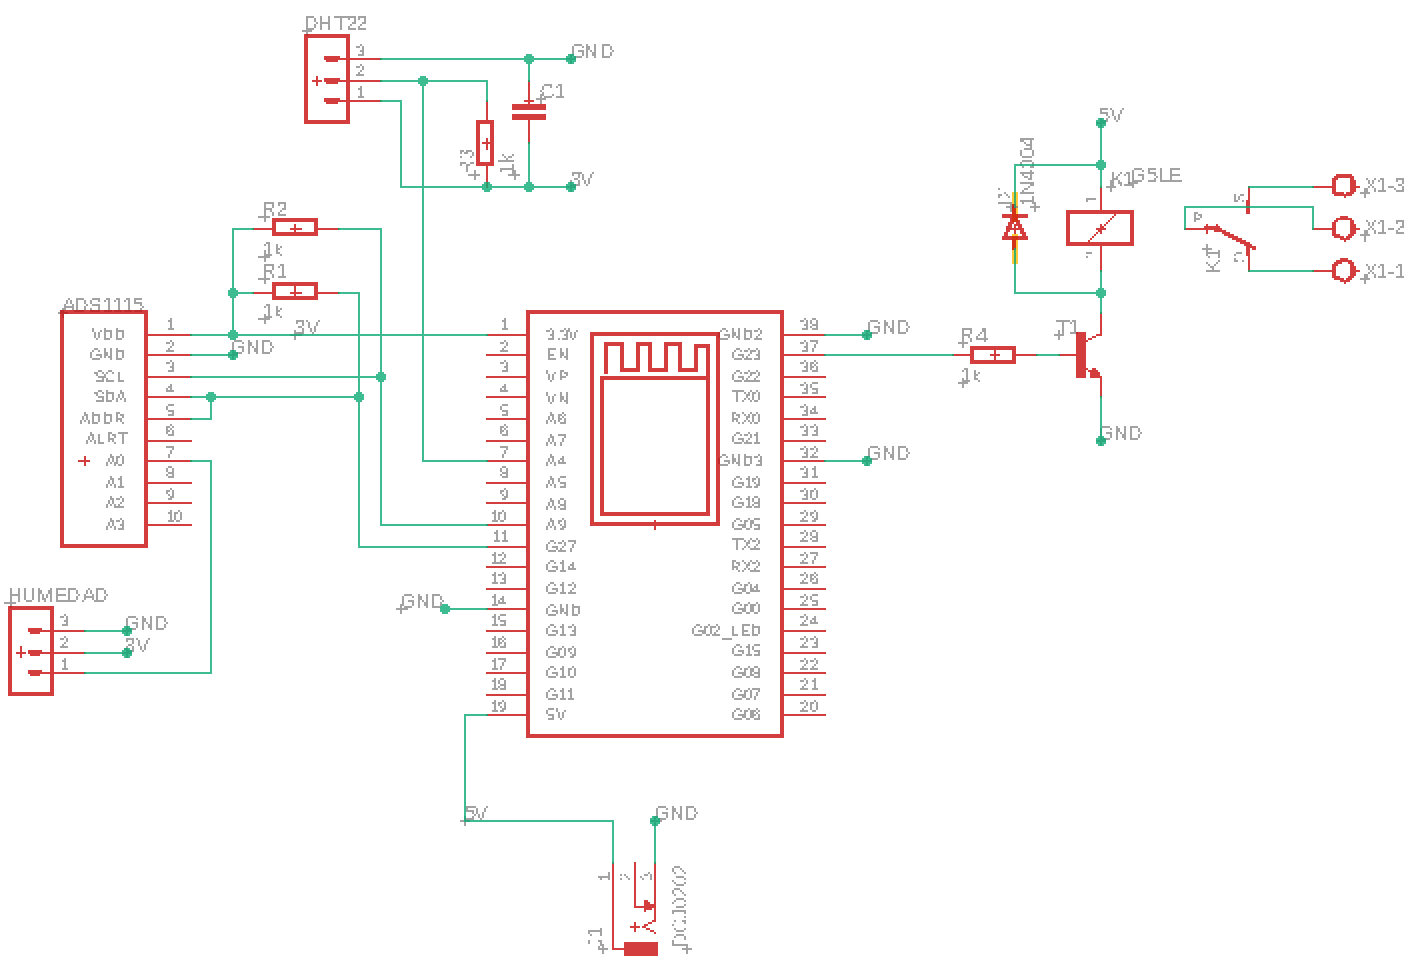
\includegraphics[width=.7\textwidth]{./Figuras/diagDipos.png}
\caption{Diagrama del prototipo.}
\label{fig:diagDipos}
\end{figure}

\vspace{25px}

\end{consigna}

\begin{consigna}{black}

Con respecto al punto 2, se trabajará en torno primer entregable del sistema de control y monitoreo. Este desarrollo se está llevando adelante con los estudiantes Guido Contento y Luciano Otegui. Dicho equipo tiene como foco finalizar la estructura base del Backend y Frontend con las altas, bajas y modificaciones de las secciones iniciales del sistema. También se realizará la primera propuesta de integración con los dispositivos. El resto de las funcionalidades quedará en el marco de trabajo del proyecto.

Finalmente, sobre el punto 3, se quiere montar una huerta en la escuela de oficios Felipe Vallese. La expectativa es que cuente con tres sectores que tengan los dispositivos de medición. Para lograr esto se debe completar un plano de la huerta. En él, se diagramará la distribución de los sectores y la ubicación de los dispositivos. Esto último, más la adquisición de los materiales, forma parte del alcance de la presente documentación.

%\vspace{25px}

\begin{figure}[htpb]
\centering 
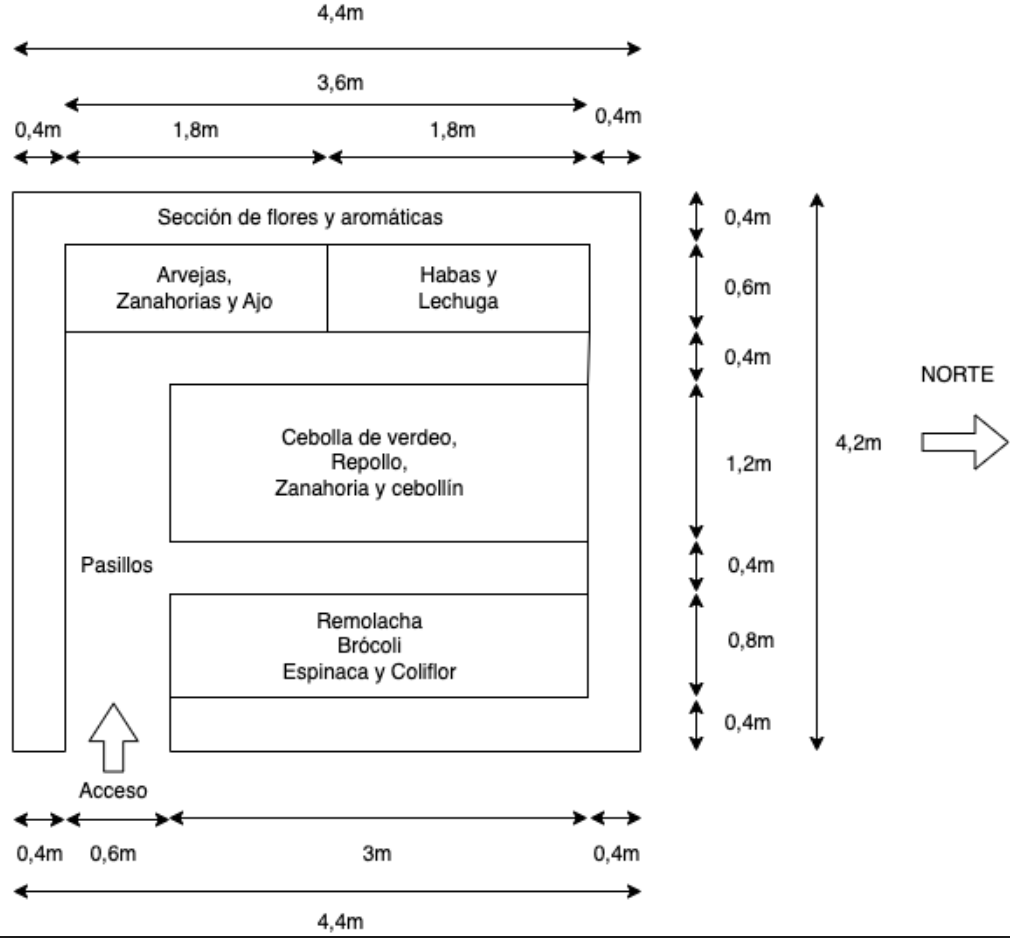
\includegraphics[width=.7\textwidth]{./Figuras/diagHuerta.png}
\caption{Plano alto nivel la huerta.}
\label{fig:diagHuerta}
\end{figure}

\vspace{25px}

No forma parte del alcance el armado en sí de la huerta, ni de su cableado eléctrico y tuberías de agua. Esta parte del trabajo la realizarán los empleados de Felipe Vallese.

\end{consigna}


\section{5. Supuestos del proyecto}
\label{sec:supuestos}

\begin{consigna}{black}
Para el desarrollo del presente proyecto se supone que:

\begin{itemize}
	\item 1: no habrá inconvenientes con el armado de la huerta por parte del equipo de Felipe Vallese.
	\item 2: las condiciones de acceso a la red de electricidad y agua serán correctas.
	\item 3: la conectividad Wi-Fi será viable en el espacio de la huerta.
	\item 4: se podrá contar con el presupuesto acordado para la compra de materiales e insumos.
	\item 5: este proyecto seguirá formando parte los trabajos de investigación prioritarios para la UNLa, por lo menos hasta fines del año 2023.
\end{itemize}
\end{consigna}

\section{6. Requerimientos}
\label{sec:requerimientos}

Los requerimientos del proyecto están agrupados por afinidad:

\begin{enumerate}
	\item Requerimientos del dispositivo
		\begin{enumerate}
			\item Debe tener un código interno para ser identificado unívocamente en el software de control.
			\item Debe contar con una placa ESP32 más dos sensores de humedad (uno de ambiente y otro de suelo).
			\item La placa ESP32 debe usar los sensores para medir los porcentajes correspondientes de las plantas de su sector. 
			\item Debe centralizar las métricas obtenidas y contar con Wi-Fi para trasmitirlas a un servidor. 
			\item Tiene que poder activar la apertura o cierre de una válvula de agua usando un comando interno.
		\end{enumerate}
	
	\item Requerimientos de integración del backend del software
		\begin{enumerate}
			\item Debe contar con un endpoint rest API para consultar las mediciones de un dispositivo.
			\item Debe contar con un endpoint rest API para solicitar a un dispositivo la apertura de la válvula de agua durante 30 segundos.
			\end{enumerate}

	\item Requerimientos del sistema para los usuarios
		\begin{enumerate}
			\item Debe permitir a un usuario loguearse al sistema usando su mail y constraseña.
			\item Debe permitir a un usuario desloguearse del sistema.
			\item Debe permitir a un usuario recuperar y cambiar su contraseña.
			\item Debe tener una sección de visualización y modificación de los datos de perfil del usuario logueado.
			\item Debe contemplar permisos para cada rol del sistema:
			\begin{enumerate}
			\item Administrador: acceso todas las funcionalidades.
			\item Responsable: acceso a las funcionalidades de administración de sus huertas.
			\item Visitante: acceso a las funcionalidades de visualización de sus huertas asociadas.
			\end{enumerate}
			\item Debe tener una sección para ver, modificar y eliminar huertas del sistema.
			\item Debe tener una sección para ver, modificar y eliminar usuarios del sistema.
			\item Debe tener una sección para administrar huertas vinculando el código de un dispositivo por sector.
			\item Debe tener una sección para administrar los porcentajes de aceptación de humedad por sector.
			\item Debe tener una sección para visualizar las mediciones de un dispositivo por sector.
			\item Debe tener una sección para ver, modificar y eliminar usuarios con rol visitante para una huertas.
			\item Debe tener una sección para ver, modificar y eliminar roles del sistema.
			\item Debe tener una sección para asociar un rol a un usuario nuevo.
			\item Debe permitir que un usuario (con rol responsable) solicite su alta en el sistema usando mail y password.
		\end{enumerate}		
		
	\item Requerimientos no funcionales
		\begin{enumerate}
			\item El sistema deberá tener un usuario administrador por defecto.
			\item Cada dispositivo deberá instalarse en un sector correctamente delimitado de la huerta.
			\item La huerta va a contar con sectores con platas que tengan características de cuidado similares.
		\end{enumerate}
		
\end{enumerate}

\section{7. Historias de usuarios (\textit{Product backlog})}
\label{sec:backlog}

Ponderación: se utiliza la sucesión de Fibonacci.
\newline Priorización: se puntúa usando una prioridad de 1 (alta) a 5 (baja).

\begin{itemize}
	\item Como usuario general quiero loguearme al sistema web usando mail y contraseña.
	\newline Ponderación: 1.
	\newline Priorización: 2.
	\item Como usuario general quiero desloguearme del sistema web.
	\newline Ponderación: 1.
	\newline Priorización: 2.
	\item Como usuario general del sistema quiero recuperar y cambiar mi contraseña.
	\newline Ponderación: 3.
	\newline Priorización: 2.
	\item Como usuario general del sistema quiero ver y editar mi información de perfil.
	\newline Ponderación: 2.
	\newline Priorización: 3.

	\item Como administrador quiero dar de alta usuarios de tipo responsable y visitante.
	\newline Ponderación: 2.
	\newline Priorización: 2.
	\item Como administrador quiero modificar o eliminar usuarios de tipo responsable y visitante.
	\newline Ponderación: 2.
	\newline Priorización: 2.
	\item Como administrador quiero dar de alta una huerta y asociarla a un responsable.
	\newline Ponderación: 5.
	\newline Priorización: 1.
	\item Como administrador quiero modificar y eliminar cualquier huerta del sistema.
	\newline Ponderación: 3.
	\newline Priorización: 2.	
	\item Como administrador quiero asociar un sector, de una huerta, a un dispositivo usando su código único.
	\newline Ponderación: 3.
	\newline Priorización: 1.
	\item Como administrador quiero crear y editar los porcentajes de aceptación de humedad por sector en cualquier huerta.
	\newline Ponderación: 3.
	\newline Priorización: 1.
	\item Como administrador quiero ver y modificar los datos básicos de los roles del sistema.
	\newline Ponderación: 2.
	\newline Priorización: 3.
	\item Como administrador quiero visualizar las mediciones de un sector de cualquier huerta.
	\newline Ponderación: 5.
	\newline Priorización: 2.
	
	\item Como responsable quiero darme de alta en el sistema con mail y password.
	\newline Ponderación: 2.
	\newline Priorización: 1.
	\item Como responsable quiero dar de alta una huerta y que se asocie a mi usuario.
	\newline Ponderación: 3.
	\newline Priorización: 1.
	\item Como responsable quiero ver, modificar y eliminar mis huertas asociadas.
	\newline Ponderación: 3.
	\newline Priorización: 2.
	\item Como responsable quiero asociar un sector, de una mis huertas, a un dispositivo usando su código único.
	\newline Ponderación: 1.
	\newline Priorización: 1.
	\item Como responsable quiero administrar los porcentajes de aceptación de humedad por sector en mis huertas.
	\newline Ponderación: 1.
	\newline Priorización: 1.
	\item Como responsable quiero visualizar las mediciones de un sector de cualquiera de mis huertas.
	\newline Ponderación: 1.
	\newline Priorización: 1.
	\item Como responsable quiero crear usuarios con rol visitante y asociarlos a cualquiera de mis huertas.
	\newline Ponderación: 2.
	\newline Priorización: 3.
	
	\item Como usuario visitante quiero visualizar las huertas a las que estoy asociado.
	\newline Ponderación: 1.
	\newline Priorización: 1.
	\item Como usuario visitante quiero visualizar las métricas de un sector de cualquiera de las huertas a las que estoy asociado.
	\newline Ponderación: 1.
	\newline Priorización: 1.
\end{itemize}


\section{8. Entregables principales del proyecto}
\label{sec:entregables}

\begin{itemize}
	\item Manual de uso.
	\item Diagrama de los esquemático del sistema global.
	\item Diagrama de los componentes de un dispositivo.
	\item Diagrama de clases del software.
	\item Manual de armado e instalación del dispositivo.
	\item Repositorio con el código fuente.
	\item Informe final.
\end{itemize}

\section{9. Desglose del trabajo en tareas}
\label{sec:wbs}

\begin{enumerate}
\item Planificación del proyecto. (55 h)
	\begin{enumerate}
	\item Definición de equipos y tareas. (5 h)
	\item Definición del comportamiento del dispositivo. (20 h)
	\item Definición del comportamiento del software. (20 h)
	\item Definición de la integración entre el dispositivo y el software. (10 h)
	\end{enumerate}
	
\item Investigación y armado del prototipo del dispositivo. (115 h)
	\begin{enumerate}
	\item Investigación de componentes. (10 h)
	\item Integración de la placa ESP32 con los sensores de humedad. (10 h)
	\item Montado del dispositivo. (20 h)
	\item Programación del dispositivo para autenticarse con el back-end del server. (10 h)
	\item Programación del dispositivo para comunicarse con el back-end del sistema. (20 h)
	\item Programación del dispositivo para centralizar las métricas obtenidas de los sensores. (15 h)
	\item Programación para apertura y cierre de la válvula de agua. (15 h)
	\item Pruebas de integración. (15 h)
	\end{enumerate}
	
\item Desarrollo del back-end del software. (180 h)
	\begin{enumerate}
	\item Modelado del diagrama de clases. (20 h)
	\item Desarrollo a arquitectura base del back-end. (15 h)
	\item Desarrollo de endpoints de gestión de usuarios y roles. (20 h)
	\item Desarrollo de endpoints de gestión permisos. (20 h)
	\item Desarrollo de endpoints de alta y baja de huertas. (25 h)
	\item Desarrollo del endpoint de modificación de huertas. (15 h)
	\item Desarrollo de endpoints de administración de una huerta. (20 h)
	\item Desarrollo de endpoints de visualización de métricas. (20 h)
	\item Desarrollo de endpoints de integración con dispositivos. (25 h)
	\end{enumerate}
	
\item Desarrollo del front-end del software. (180 h)
	\begin{enumerate}
	\item Maquetado de las vistas generales del sitio web con la definición de estilos y colores. (25 h)
	\item Desarrollo de la arquitectura base del front-end. (15 h)
	\item Desarrollo de la vista gestión de usuarios y roles. (30 h)
	\item Desarrollo de las vistas de alta y baja de huertas. (20 h)
	\item Desarrollo de la vista de modificación de huertas. (20 h)
	\item Desarrollo de las vistas de administración de una huerta. (20 h)
	\item Desarrollo de la vista para visualización de métricas de la semana completa. (25 h)
	\item Desarrollo de la vista para visualización de métricas en tiempo real. (25 h)
	\end{enumerate}

\item Documentación del proyecto. (70 h)
	\begin{enumerate}
	\item Armando del informe de avance. (10 h)
	\item Armando de la memoria del proyecto. (30 h)
	\item Correcciones de documentos en base a las revisiones. (10 h)
	\item Elaboración de la presentación final. (20 h)
	\end{enumerate}	
	
\end{enumerate}

Cantidad total: 600 horas.

\section{10. Diagrama de Activity On Node}
\label{sec:AoN}

Código de colores por grupo de tareas:
\begin{itemize}
	\item Celeste: proceso de inicio o fin.
	\item Verde: planificación del proyecto.
	\item Amarillo: investigación y armado del prototipo del dispositivo.
	\item Violeta: desarrollo del back-end del software.
	\item Rojo: desarrollo del front-end del software. 
	\item Gris: Documentación del proyecto.
\end{itemize}

En cada tarea la letra 't' representa el tiempo total de trabajo estimado en horas.

\begin{figure}[htpb]
\centering 
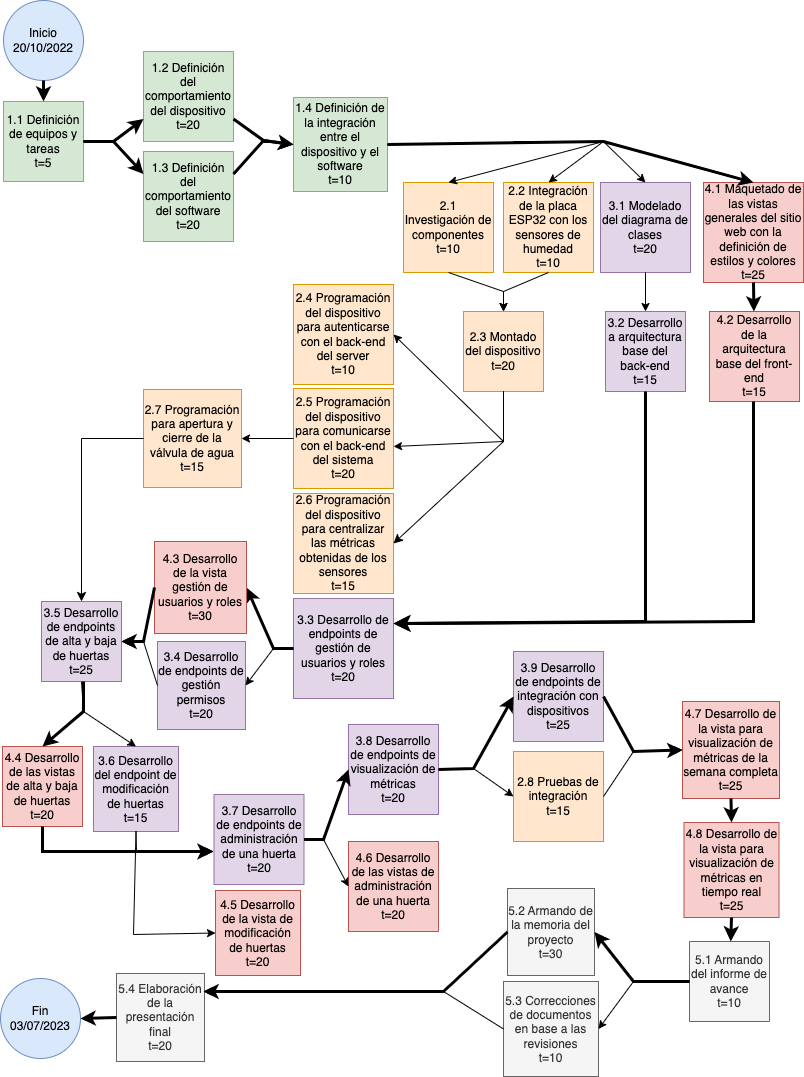
\includegraphics[width=.9\textwidth]{./Figuras/AoN.png}
\caption{Diagrama en \textit{Activity on Node}.}
\label{fig:AoN}
\end{figure}

\section{11. Diagrama de Gantt}
\label{sec:gantt}

Consideraciones del Gantt:
\begin{itemize}
\item Para su desarrollo se utilizó la herramienta Trello con el plugin BigPicture.
\item Aunque se cuenta con una imagen completa del Gannt en el presente documento figura en dos partes. Esto se debe a que la línea de tiempo es muy larga y se optó por facilitar su lectura. Cada parte contempla 4 meses de trabajo en la planificación.
\item De igual forma, en pos de mejorar su legibilidad, se agregan ambas partes del Gantt en formato horizontal.
\item Solo existe un recurso asignado ya que el resto del equipo finalizó sus tareas y colaboraciones.
\item Durante el mes de enero 2023 no se va a trabajar. Por ello para ese periodo se definió una tarea como "Day off. Vacaciones".
\item Para estimar el tiempo de cada tarea se tuvo en cuenta un promedio de trabajo entre 2 y 4 horas en días de semana. A su vez se tuvieron en cuenta los días feriados en la estimación.
\end{itemize}

\begin{landscape}
\begin{figure}[htpb]
\centering 
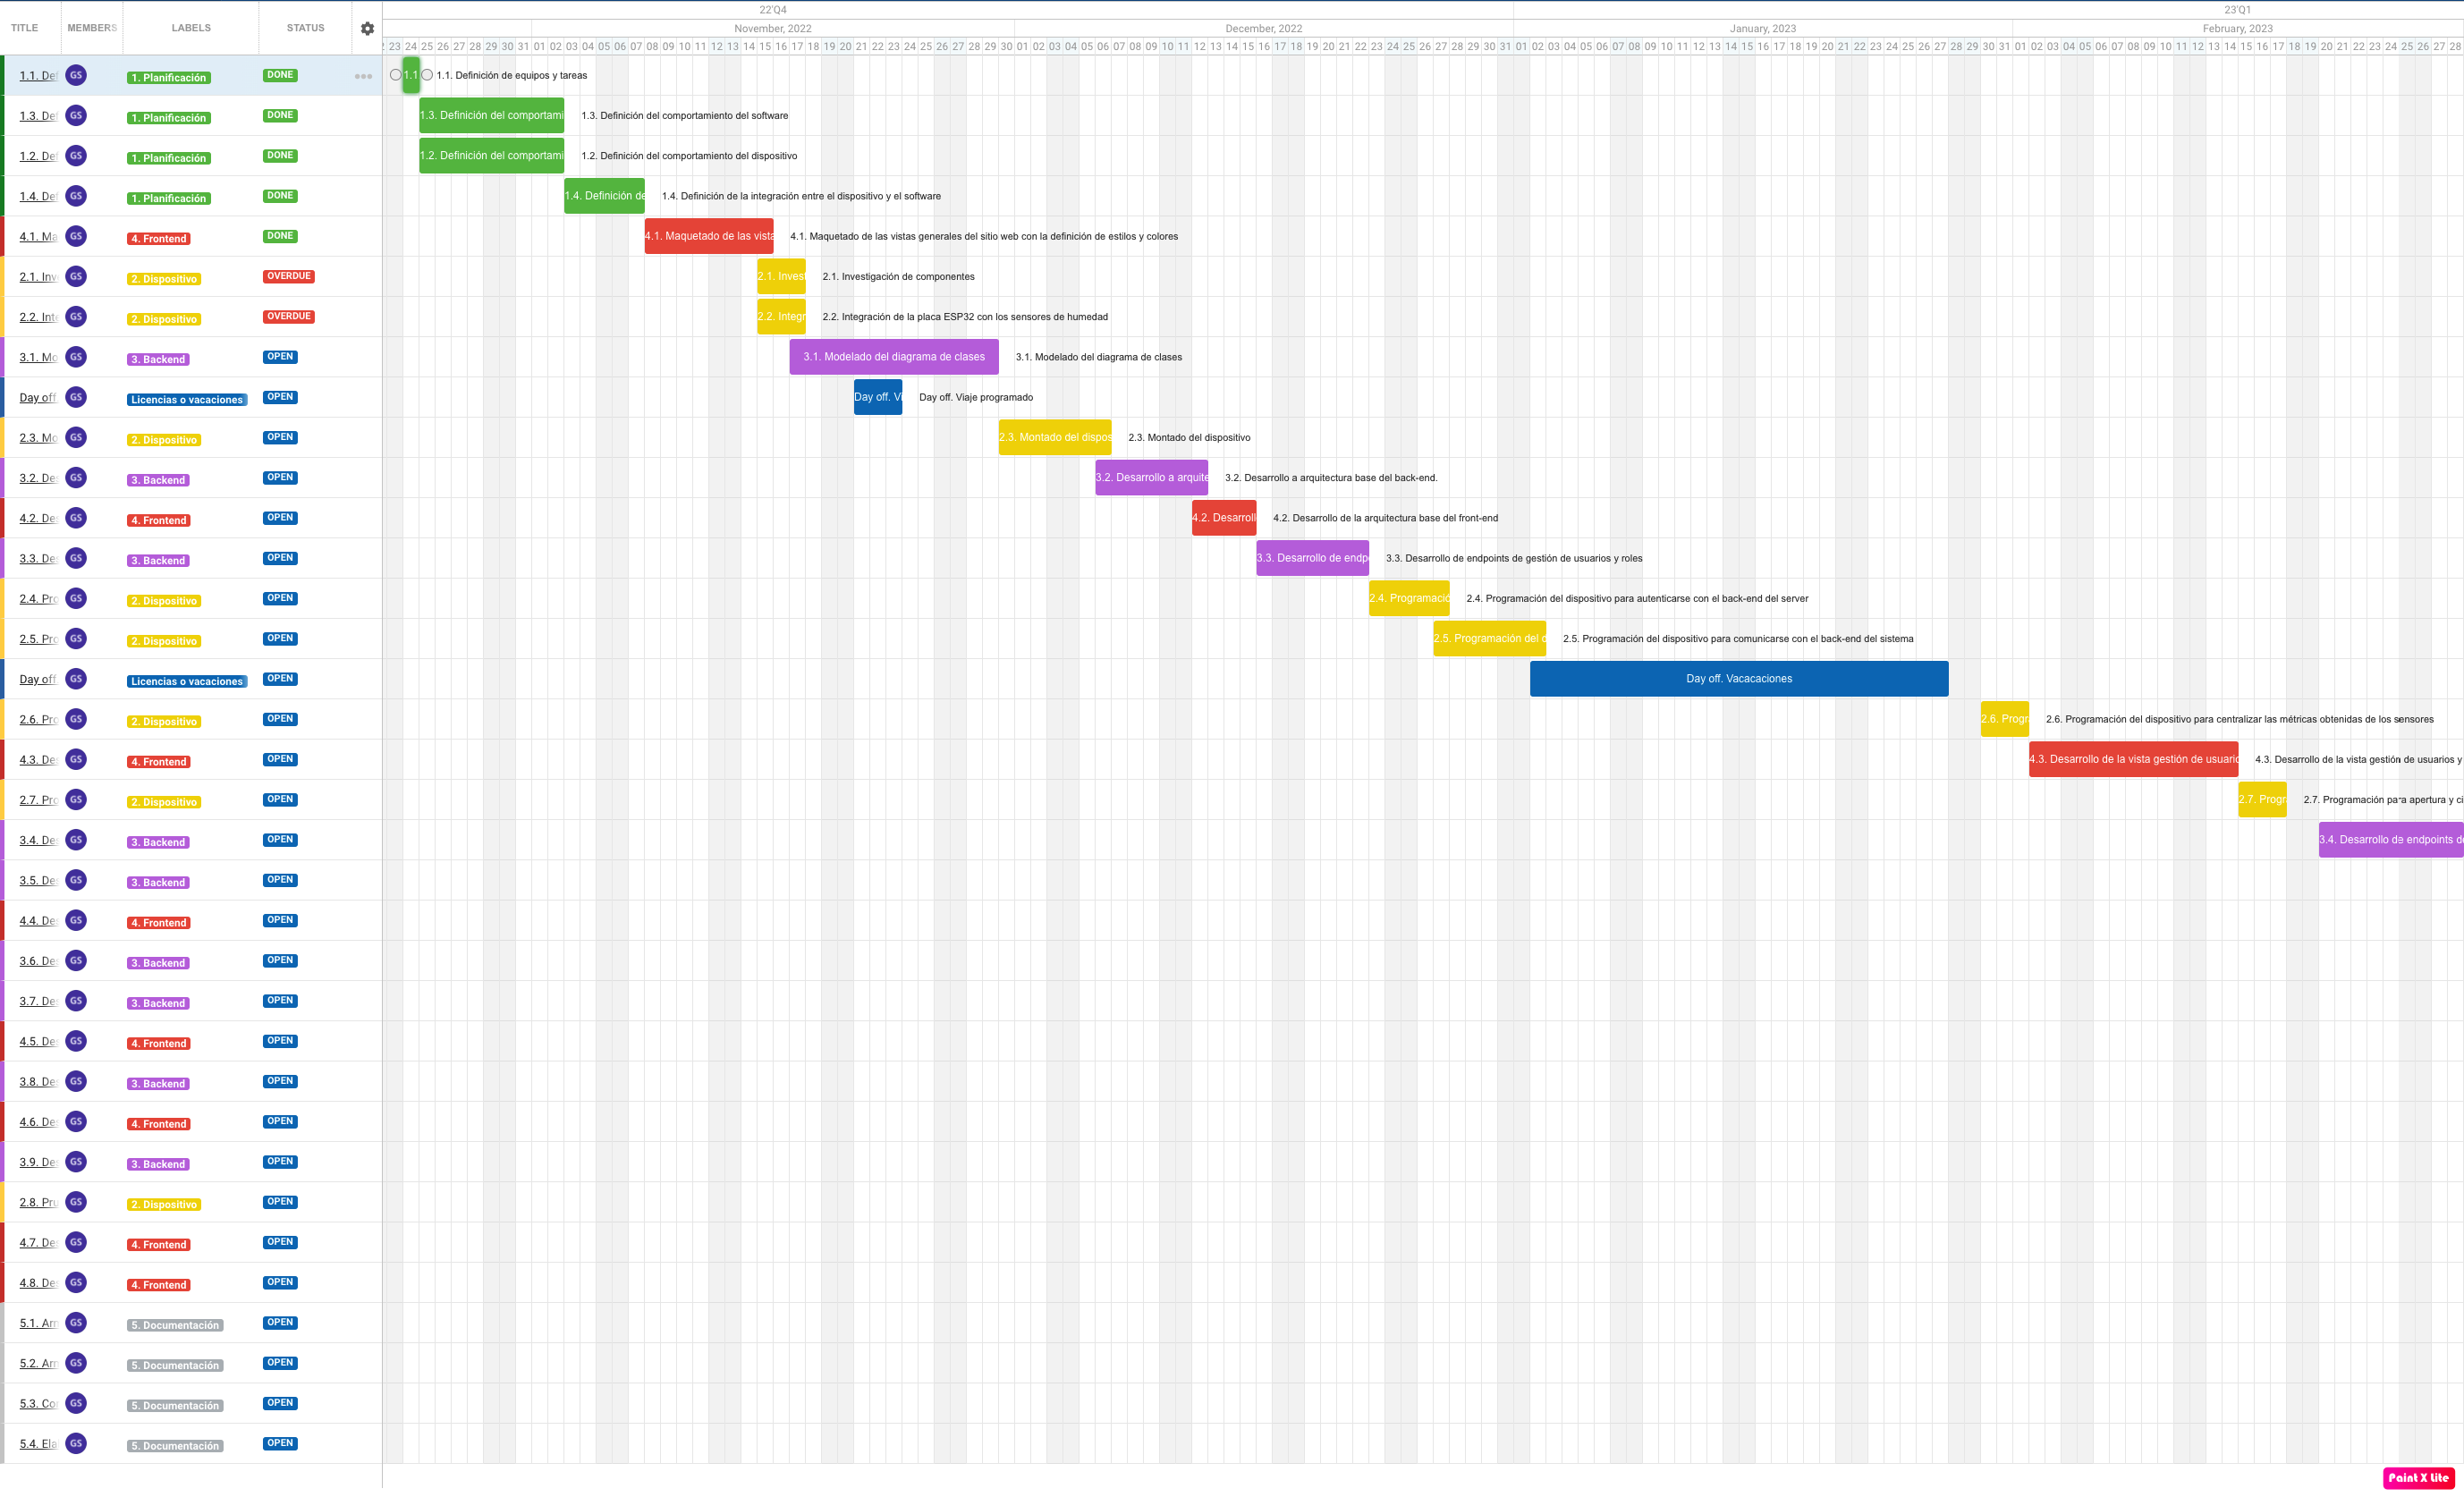
\includegraphics[height=.95\textheight]{./Figuras/Gantt-parte1-2.png}
\caption{Diagrama de Gantt parte 1/2}
\label{fig:diagGantt1-2}
\end{figure}
\end{landscape}

\begin{landscape}
\begin{figure}[htpb]
\centering 
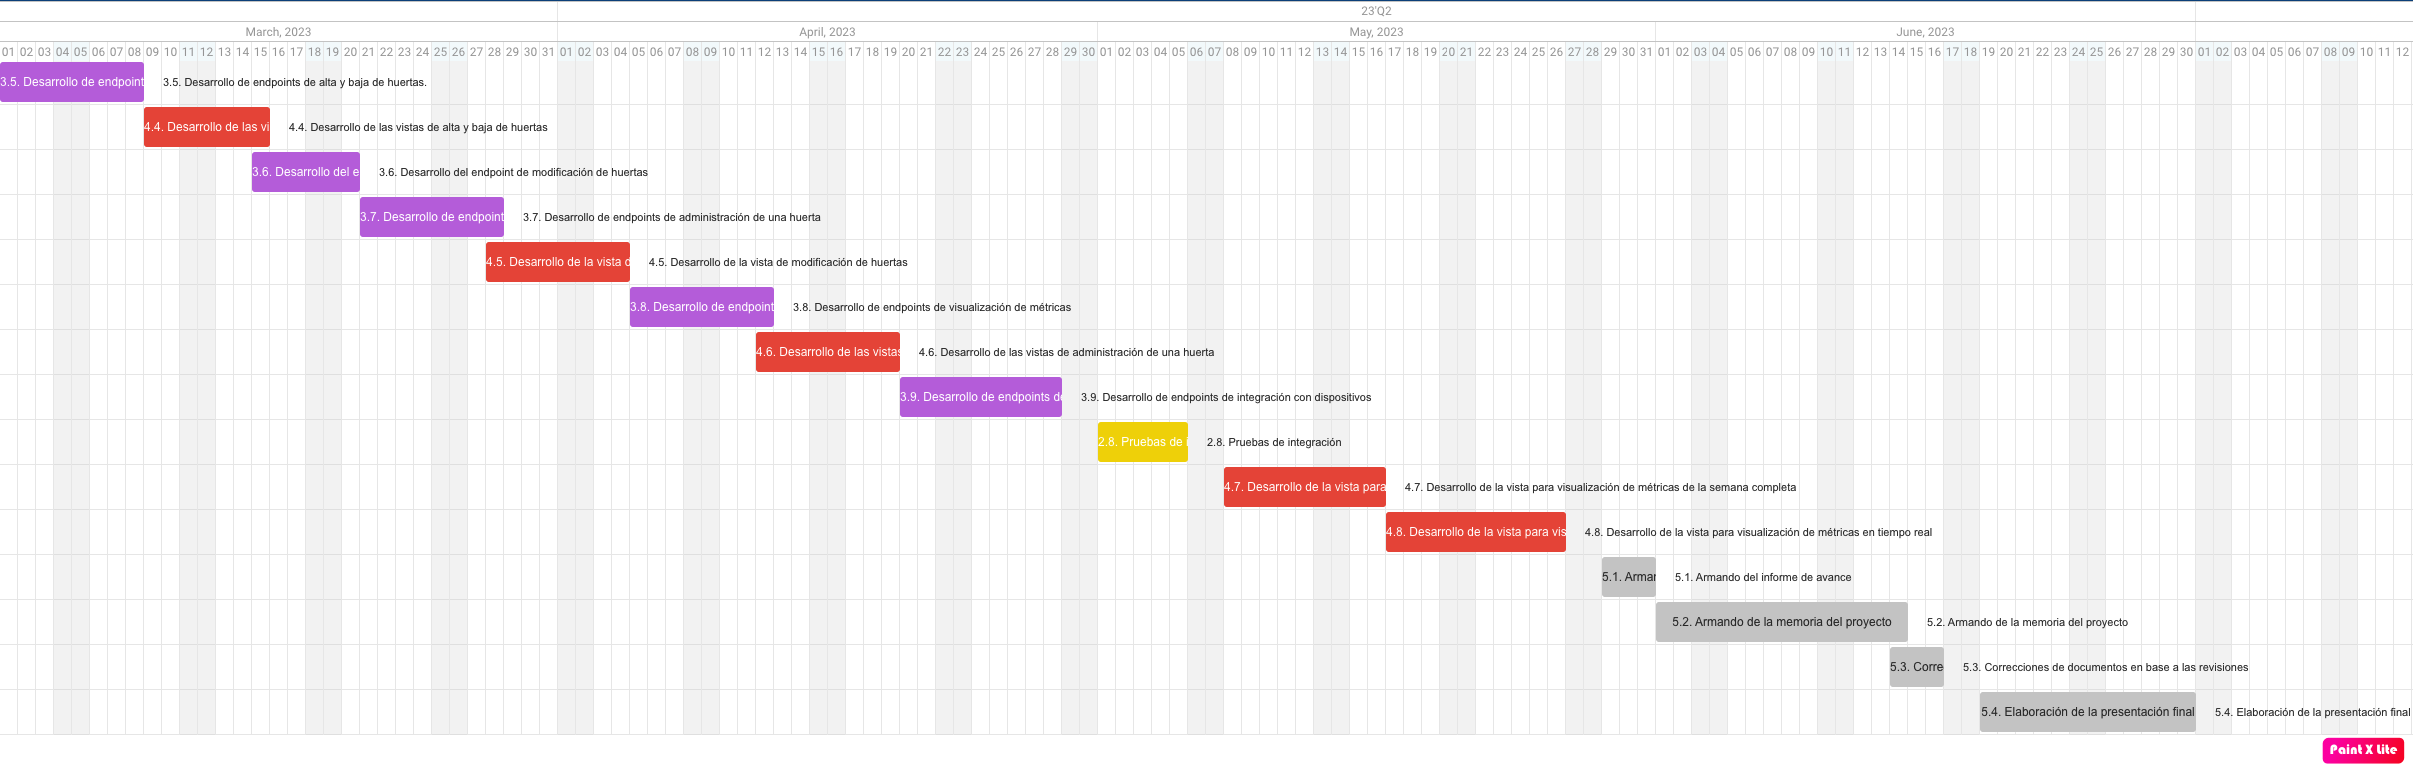
\includegraphics[height=.5\textheight]{./Figuras/Gantt-parte2-2.png}
\caption{Diagrama de Gantt parte 2/2}
\label{fig:diagGantt2-2}
\end{figure}
\end{landscape}

\section{12. Presupuesto detallado del proyecto}
\label{sec:presupuesto}

Los valores en el presupuesto están expresados en pesos argentinos.

\begin{table}[htpb]
\centering
\begin{tabularx}{\linewidth}{@{}|X|c|r|r|@{}}
\hline
\rowcolor[HTML]{C0C0C0} 
\multicolumn{4}{|c|}{\cellcolor[HTML]{C0C0C0}COSTOS DIRECTOS} \\ \hline
\rowcolor[HTML]{C0C0C0} 
Descripción &
  \multicolumn{1}{c|}{\cellcolor[HTML]{C0C0C0}Cantidad} &
  \multicolumn{1}{c|}{\cellcolor[HTML]{C0C0C0}Valor unitario} &
  \multicolumn{1}{c|}{\cellcolor[HTML]{C0C0C0}Valor total} \\ \hline
  
 NodeMCU ESP32&
  \multicolumn{1}{c|}{4} &
  \multicolumn{1}{c|}{\$3.000} &
  \multicolumn{1}{c|}{\$12.000} \\ \hline

 Sensor de temperatura y humedad relativa DHT11&
  \multicolumn{1}{c|}{1} &
  \multicolumn{1}{c|}{\$500} &
  \multicolumn{1}{c|}{\$500} \\ \hline

 Sensor de humedad en suelo capacitivo analógico V1.2 Premium&
  \multicolumn{1}{c|}{4} &
  \multicolumn{1}{c|}{\$1.141} &
  \multicolumn{1}{c|}{\$4.564} \\ \hline

 ADC ADS1115&
  \multicolumn{1}{c|}{1} &
  \multicolumn{1}{c|}{\$2.990} &
  \multicolumn{1}{c|}{\$2.990} \\ \hline

 Fabricación PCB 56x75 mm una capa&
  \multicolumn{1}{c|}{4} &
  \multicolumn{1}{c|}{\$1.500} &
  \multicolumn{1}{c|}{\$6.000} \\ \hline

 Cable usb a micro usb 1 metro&
  \multicolumn{1}{c|}{4} &
  \multicolumn{1}{c|}{\$290} &
  \multicolumn{1}{c|}{\$1.160} \\ \hline

 Cargador portátil celular&
  \multicolumn{1}{c|}{4} &
  \multicolumn{1}{c|}{\$400} &
  \multicolumn{1}{c|}{\$1.600} \\ \hline

 Resistencias 1 k 1/4 w&
  \multicolumn{1}{c|}{16} &
  \multicolumn{1}{c|}{\$12} &
  \multicolumn{1}{c|}{\$192} \\ \hline

 Jack alimentación DCJ0202&
  \multicolumn{1}{c|}{4} &
  \multicolumn{1}{c|}{\$110} &
  \multicolumn{1}{c|}{\$440} \\ \hline
 
 Plug alimentación&
  \multicolumn{1}{c|}{4} &
  \multicolumn{1}{c|}{\$50} &
  \multicolumn{1}{c|}{\$200} \\ \hline
 
 Conectores molex de 3 pines&
  \multicolumn{1}{c|}{4} &
  \multicolumn{1}{c|}{\$26} &
  \multicolumn{1}{c|}{\$104} \\ \hline

 Transistor 2n2222&
  \multicolumn{1}{c|}{4} &
  \multicolumn{1}{c|}{\$42} &
  \multicolumn{1}{c|}{\$168} \\ \hline

 Diodo 1N4004&
  \multicolumn{1}{c|}{4} &
  \multicolumn{1}{c|}{\$54} &
  \multicolumn{1}{c|}{\$216} \\ \hline

 Capacitor 100 nf&
  \multicolumn{1}{c|}{4} &
  \multicolumn{1}{c|}{\$37} &
  \multicolumn{1}{c|}{\$148} \\ \hline

 Tira 40 pines&
  \multicolumn{1}{c|}{6} &
  \multicolumn{1}{c|}{\$107} &
  \multicolumn{1}{c|}{\$642} \\ \hline

 Caja estanca 20x20x10&
  \multicolumn{1}{c|}{4} &
  \multicolumn{1}{c|}{\$1.095} &
  \multicolumn{1}{c|}{\$4.380} \\ \hline

 Caja estanca 11, 5x11, 5x60&
  \multicolumn{1}{c|}{4} &
  \multicolumn{1}{c|}{\$256} &
  \multicolumn{1}{c|}{\$1.024} \\ \hline

Válvula solenoide 220 V de lavarropas&
  \multicolumn{1}{c|}{4} &
  \multicolumn{1}{c|}{\$1.050} &
  \multicolumn{1}{c|}{\$4.200} \\ \hline

 Relay 5 V 10 A&
  \multicolumn{1}{c|}{4} &
  \multicolumn{1}{c|}{\$610} &
  \multicolumn{1}{c|}{\$2.440} \\ \hline
  
 Cable subterráneo 2x2,5 mm x 25 m&
  \multicolumn{1}{c|}{20} &
  \multicolumn{1}{c|}{\$260} &
  \multicolumn{1}{c|}{\$5.200} \\ \hline
  
  Cable UTP5 por 50 m&
  \multicolumn{1}{c|}{10} &
  \multicolumn{1}{c|}{\$54} &
  \multicolumn{1}{c|}{\$540} \\ \hline
  
  Manguera microperforada por 15 m &
  \multicolumn{1}{c|}{9} &
  \multicolumn{1}{c|}{\$267} &
  \multicolumn{1}{c|}{\$2.403} \\ \hline
  
   Conector T manguera 1/2&
  \multicolumn{1}{c|}{10} &
  \multicolumn{1}{c|}{\$629} &
  \multicolumn{1}{c|}{\$6290} \\ \hline
  
  Caño PVC 40x1, 8 mm x 4 m reforzado &
  \multicolumn{1}{c|}{4} &
  \multicolumn{1}{c|}{\$1.109} &
  \multicolumn{1}{c|}{\$4436} \\ \hline 
    
\multicolumn{3}{|c|}{SUBTOTAL} &
  \multicolumn{1}{c|}{\$61.837} \\ \hline
\rowcolor[HTML]{C0C0C0} 
\multicolumn{4}{|c|}{\cellcolor[HTML]{C0C0C0}COSTOS INDIRECTOS} \\ \hline
\rowcolor[HTML]{C0C0C0} 
Descripción &
  \multicolumn{1}{c|}{\cellcolor[HTML]{C0C0C0}Cantidad} &
  \multicolumn{1}{c|}{\cellcolor[HTML]{C0C0C0}Valor unitario} &
  \multicolumn{1}{c|}{\cellcolor[HTML]{C0C0C0}Valor total} \\ \hline
\multicolumn{1}{|l|}{30 \%  de los costos directos} &
  {1} &
  {\$18.551,1} &
  {\$18.551,1} \\ \hline
\multicolumn{3}{|c|}{SUBTOTAL} &
  \multicolumn{1}{c|}{\$18.551,1} \\ \hline
\rowcolor[HTML]{C0C0C0}
\multicolumn{3}{|c|}{TOTAL} & \$80.388,1
   \\ \hline
\end{tabularx}%
\end{table}


\section{13. Gestión de riesgos}
\label{sec:riesgos}
 
Riesgo 1: no contar los materiales a tiempo para el prototipo en la huerta.
\begin{itemize}
	\item Severidad (S): 8.
	Esto va a demorar las pruebas de software y podría generar retrasos en todas las etapas.
	\item Probabilidad de ocurrencia (O): 5.
	Hay una probabilidad intermedia de no poder comprar todos los materiales a tiempo. 
\end{itemize}   

Riesgo 2: no contar con el presupuesto asignado del proyecto.
\begin{itemize}
	\item Severidad (S): 10.
	Si esto sucede se para todo el proyecto.
	\item Ocurrencia (O): 3.
	Según lo acordado con la Universidad esto es poco probable.
\end{itemize}

Riesgo 3: no contar con buena señal de internet en la huerta.
\begin{itemize}
	\item Severidad (S): 5.
	En caso de que no se cuente con buena señal de internet no se van a poder enviar las métricas al servidor.
	\item Ocurrencia (O): 2.
	Según lo acordado con la Universidad esto es poco probable.
\end{itemize}

Riesgo 4: no contar con la infraestructura de electricidad y agua en la huerta.
\begin{itemize}
	\item Severidad (S): 10.
	Esto haría que el proyecto en sí no tenga sentido porque no se podría cumplir el objetivo del cuidado de la huerta.
	\item Ocurrencia (O): 1.
	Según lo acordado con la Universidad esto no es probable.
\end{itemize}

Riesgo 5: No alcanzar los conocimientos necesarios para el desarrollo en la placa, el backend y el frontend.
\begin{itemize}
	\item Severidad (S): 7.
	En caso no tener un buen conocimiento para el desarrollo el proyecto va a ser inestable, lo que podría generar demoras en las entregas y problemas con la liquidación presupuesto.
	\item Ocurrencia (O): 3.
	Se espera cubrir todo lo necesario en la especialización más cursos extras.
\end{itemize}

b) Tabla de gestión de riesgos:      (El RPN se calcula como RPN=SxO)

\begin{table}[htpb]
\centering
\begin{tabularx}{\linewidth}{@{}|X|c|c|c|c|c|c|@{}}
\hline
\rowcolor[HTML]{C0C0C0} 
Riesgo & S & O & RPN & S* & O* & RPN* \\ \hline
      No contar los materiales a tiempo para el prototipo en la huerta &   8&   5&     40&    8&    2& 16     \\ \hline
      No contar con el presupuesto asignado del proyecto &   10&   3&     30&   10 &   2 & 20     \\ \hline
      No contar con buena señal de internet en la huerta &   5&   2&     10&   - &  -  & -     \\ \hline
      No contar con la infraestructura de electricidad y agua en la huerta &  10 &   1&     10&    -&  -  & -     \\ \hline
      No alcanzar los conocimientos necesarios para el desarrollo en la placa, el backend y el frontend &  7 &  3 & 21 &   - &   - &  -    \\ \hline
\end{tabularx}%
\end{table}

Criterio adoptado: 
Se tomarán medidas de mitigación en los riesgos cuyos números de RPN sean mayores a 25.

Nota: los valores marcados con (*) en la tabla corresponden luego de haber aplicado la mitigación.

c) Plan de mitigación de los riesgos que originalmente excedían el RPN máximo establecido:
 
Riesgo 1: no contar los materiales a tiempo para el prototipo en la huerta.
\begin{itemize}
	\item Plan de mitigación: se va a planificar la compra de materiales para la segunda semana de diciembre y se buscará un mínimo de 3 locales diferentes para tener varias opciones a la hora de realizar las compras.
	\item Severidad (S*): 8. Se mantiene el mismo criterio.
	\item Probabilidad de ocurrencia (O*): 2. Los materiales deberían que ser fáciles de conseguir en diferentes locales.
\end{itemize}
Riesgo 2: no contar con el presupuesto asignado del proyecto.
\begin{itemize}
	\item Plan de mitigación: con la planificación anterior se va a generar una reunión con la Universidad para acordar las fechas de liquidación del presupuesto, de esa forma se podrá acordar su uso a tiempo.
	\item Severidad (S*): 10. Se mantiene el mismo criterio.
	\item Probabilidad de ocurrencia (O*): 2. Desde la Universidad debería haber buena predisposición para avanzar si se cuenta con un plan detallado.
\end{itemize}

\section{14. Gestión de la calidad}
\label{sec:calidad}

Listado de requerimientos con sus verificaciones y validaciones:

\begin{itemize}
\item Requerimientos del dispositivo.
	\begin{itemize}
	\item Req \#1.1: debe tener un código interno para ser identificado unívocamente en el software de control.
		\begin{itemize}
		\item Verificación: se comprobará que el programa de la placa genere un código de forma única para un dispositivo.
		\item Validación: se realizarán pruebas en al menos dos placas para asegurarse que el código que llega al backend es diferente en cada caso.\\
		\end{itemize}
		
	\item Req \#1.2: debe contar con una placa ESP32 más dos sensores de humedad (uno de ambiente y otro de suelo).
		\begin{itemize}
		\item Verificación: se comprobará que cada componente sea el correcto verificando sus funciones.
		\item Validación: se realizarán pruebas en una placa para validar que las mediciones de cada sensor sean las correctas.\\
		\end{itemize}
		
	\item Req \#1.3: la placa ESP32 debe usar los sensores para medir los porcentajes correspondientes de las plantas de su sector.
		\begin{itemize}
		\item Verificación: se comprobará el correcto funcionamiento de cada sensor sobre la huerta.
		\item Validación: se realizarán pruebas para validar que las mediciones aumentan a medida que se agrega agua en la huerta.\\
		\end{itemize}
		 
	\item Req \#1.4: debe centralizar las métricas obtenidas y contar con Wi-Fi para trasmitirlas a un servidor.
		\begin{itemize}
		\item Verificación: se comprobará que la placa tenga la programación para tomar las métricas y transmitirlas vía Wi-Fi.
		\item Validación: se realizarán pruebas en al menos dos placas para validar que las métricas lleguen correctamente al servidor. Además se evaluará la calidad de señal de Wi-Fi con una medición de RSSI.\\
		\end{itemize}
		 
	\item Req \#1.5: tiene que poder activar la apertura o cierre de una válvula de agua usando un comando interno.
		\begin{itemize}
		\item Verificación: se comprobará que la placa tiene la programación suficiente para accionar la apertura o cierre de la válvula.
		\item Validación: se realizarán pruebas en una placa para corroborar si efectivamente esta puede abrir y cerrar la válvula.\\
		\end{itemize}
		
	\end{itemize}
	
\item Requerimientos de integración del backend del software.
	\begin{itemize}
	\item Req \#2.1: debe contar con un endpoint rest API para consultar las mediciones de un dispositivo.
		\begin{itemize}
		\item Verificación: se comprobará que el backend tiene la programación para recibir las mediciones de un dispositivo vía rest API.
		\item Validación: se realizarán pruebas desde el backend para corroborar que todas las mediciones de un dispositivo llegan correctamente.\\
		\end{itemize}
		
	\item Req \#2.2: debe contar con un endpoint rest API para solicitar a un dispositivo la apertura de la válvula de agua durante 30 segundos.
		\begin{itemize}
		\item Verificación: se comprobará que el backend tiene la programación para enviar un mensaje de apertura o cierre de la válvula a un dispositivo.
		\item Validación: se realizarán pruebas para validar que el mensaje llega y que el dispositivo lo opera correctamente.\\
		\end{itemize}
		
	\end{itemize}

\item Requerimientos del sistema para los usuarios.
	\begin{itemize}
	\item Req \#3.1: debe permitir a un usuario loguearse al sistema usando su mail y constraseña.
		\begin{itemize}
		\item Verificación: se comprobará que exista un flujo de programación que permita a un usuario loguearse.
		\item Validación: se realizarán pruebas de logueo con al menos 2 usuarios.\\
		\end{itemize}
		
	\item Req \#3.2: debe permitir a un usuario desloguearse del sistema.
		\begin{itemize}
		\item Verificación: se comprobará que exista un flujo de programación que permita a un usuario desloguearse.
		\item Validación: se realizarán pruebas de deslogueo con al menos 2 usuarios.\\
		\end{itemize}
		
	\item Req \#3.3: debe permitir a un usuario recuperar y cambiar su contraseña.
		\begin{itemize}
		\item Verificación: se comprobará que exista un flujo de programación que permita a un usuario gestionar una nueva contraseña.
		\item Validación: se realizarán pruebas al menos 3 usuarios para cambiar sus contraseñas efectivamente.\\
		\end{itemize}
		
	\item Req \#3.4: debe tener una sección de visualización y modificación de los datos de perfil del usuario logueado.
		\begin{itemize}
		\item Verificación: se comprobará que exista un flujo de programación que permita a un usuario acceder a su perfil.
		\item Validación: se realizarán pruebas con al menos 2 usuarios para validar que todos puedan acceder correctamente a su perfil.\\
		\end{itemize}
		
	\item Req \#3.5: debe contemplar permisos para cada rol del sistema.
		\begin{itemize}
		\item Verificación: se comprobará que existe un sistema de permisos tanto en el backend como en el frontend para cada tipo de usuario.
		\item Validación: se realizarán pruebas con usuarios de todos los roles del sistema para validar que cada uno pueda acceder y tener los permisos correspondientes en cada vista del frontend.\\
		\end{itemize}
		
	\item Req \#3.6: debe tener una sección para ver, modificar y eliminar huertas del sistema.
		\begin{itemize}
		\item Verificación: se comprobará que existe una vista en el frontend para modificar y eliminar huertas.
		\item Validación: se realizarán pruebas sobre la vista para modificar al menos 3 huertas y luego proceder con su correcta eliminación del sistema.\\
		\end{itemize}
		
	\item Req \#3.7: debe tener una sección para ver, modificar y eliminar usuarios del sistema.
		\begin{itemize}
		\item Verificación: se comprobará que existe una vista en el frontend para modificar y eliminar usuarios.
		\item Validación: se realizarán pruebas sobre la vista para modificar al menos 3 usuarios y luego proceder con su correcta eliminación del sistema.\\
		\end{itemize}
		
	\item Req \#3.8: debe tener una sección para administrar huertas vinculando el código de un dispositivo por sector.
		\begin{itemize}
		\item Verificación: se comprobará que existe un flujo en el sistema donde se puede vincular un dispositivo  a un sector de una huerta.
		\item Validación: se realizarán pruebas para vincular al menos 4 dispositivos en una huerta.\\
		\end{itemize}
		
	\item Req \#3.9: debe tener una sección para administrar los porcentajes de aceptación de humedad por sector.
		\begin{itemize}
		\item Verificación: se comprobará que existe una vista donde se pueden administrar los porcentajes.
		\item Validación: se realizarán pruebas para ingresar diferentes porcentajes de aceptación en al menos 3 sectores de una huerta.\\
		\end{itemize}
		
	\item Req \#3.10: debe tener una sección para visualizar las mediciones de un dispositivo por sector.
		\begin{itemize}
		\item Verificación: se comprobará que existe una vista donde se puedan ver las métricas de un sector en particular.
		\item Validación: se realizarán pruebas para validar que todas las métricas se visualicen correctamente.\\
		\end{itemize}
		
	\item Req \#3.11: debe tener una sección para ver, modificar y eliminar usuarios con rol visitante para una huertas.
		\begin{itemize}
		\item Verificación: se comprobará que existe una vista en el frontend para modificar y eliminar usuarios visitantes en una huerta.
		\item Validación:se realizarán pruebas sobre la vista para modificar al menos 3 usuarios con rol visitante y luego proceder con su correcta eliminación de la huerta.\\
		\end{itemize}
		
	\item Req \#3.12: debe tener una sección para ver, modificar y eliminar roles del sistema.
		\begin{itemize}
		\item Verificación: se comprobará que existe una vista en el frontend para modificar y eliminar los roles del sistema.
		\item Validación:se realizarán pruebas sobre la vista para modificar al menos 3 roles y luego proceder con su correcta eliminación del sistema.\\
		\end{itemize}
		
	\item Req \#3.13: debe tener una sección para asociar un rol a un usuario nuevo.
		\begin{itemize}
		\item Verificación: se comprobará que existe un flujo en el cual se pueda agregar un rol a un usuario.
		\item Validación: se realizarán pruebas para agregar roles a al menos 3 usuarios diferentes.\\
		\end{itemize}
		
	\item Req \#3.14: debe permitir que un usuario (con rol responsable) solicite su alta en el sistema usando mail y password.
		\begin{itemize}
		\item Verificación: se comprobará que existe un flujo en el cual un usuario con rol responsable puede solicitar su creación en el sistema.
		\item Validación: se realizarán pruebas para realizar dicha solicitud de forma exitosa con al menos 3 usuarios con rol responsable.
		\end{itemize}
		
\end{itemize}
\end{itemize}

\section{15. Procesos de cierre}    
\label{sec:cierre}

Al finalizar el proyecto se seguirán los siguientes pasos:

\begin{itemize}
	\item Se realizará un informe que tendrá contemplado:
	\begin{itemize}
		\item Una comparación entre los tiempos y presupuesto estimado contra lo real.
		\item Un análisis sobre las tecnologías y herramientas que se tuvieron que agregar y descartar durante el desarrollo del proyecto.
		\item Un análisis sobre el resultado técnico final.
		\item Un detalle sobre la viabilidad que hubo a la hora de montar la huerta y administrar los valores obtenidos de la misma.
	\end{itemize}
	\item Con el informe se tendrá una reunión con la directora de la carrera de la Licenciatura en Sistemas para analizar los resultados obtenidos.
	\item Posteriormente se creará una comunicación para cada involucrado en el proyecto para compartir los resultados y dar agradecimientos.
	\item Por otro lado se creará una comunicación a alto nivel para la comunidad de la Universidad Nacional de Lanús.
	\item Finalmente se realizará la defensa pública del proyecto. Esta se llevará a cabo de forma virtual y participarán los interesados, jurados y autoridades de la especialización. Al final de la presentación se agradecerá formalmente a todos aquellos que colaboraron durante el proyecto. El Acto de Cierre estará a cargo de la dirección de la carrera.	
	
	
\end{itemize}


\end{document}
